%% ----------------------------------------------------------------
%% OverallApproach.tex
%% ---------------------------------------------------------------- 
\chapter{Overall Approach} 
\label{Chapter:Overall Approach}

\begin{preamble}
To create a quality framework an overall approach for the project was decided on.

This was done by first summarising the research conducted into previous work, as well as defining where this project fits within that ecosystem. Specific requirements were gathered from the client and an analysis of the needs of other project stakeholders conducted. This led to a list of requirements that the project would need to meet. Additionally though was put into the general system design of the framework.
\end{preamble}

\section{Reviewing Previous Work}
Having reviewed the \href{Chapter:Previous Work}{previous work} some design decisions for the project could be proposed to the client:
\begin{itemize}
\item A basic quiz standard would need to be defined to allow interoperability between the authoring tool and overlaid video player. It was decided not to use the \gls{QTI} standard to define the quizzes due to the complexity and difficulty of implementing accessibility. The time constraint on this project would mean that more time would be spent on ensuring compliance with \gls{QTI} than implementing the tools.

\item One of the main features the interactive video must have is the ability to provide immediate feedback to allow for effective formative assessment to take place.

\item A HTML5 video player will be used to play the videos. This will enable mobile devices that no longer support Flash to play the interactive videos. The HTML5 control elements will simplify the implementation of keyboard accessibility.

\item The overlaid video player will need to emit events that can be captured and used to analyse the viewing patterns of the interactive videos. This would allow the viewing patterns to be compared and contrasted with traditional videos.
\end{itemize}

\section{Client Requirements}
With the end aim of integrating this project into the new version of Synote there were some specific requirements that our client had with regards to implementation.

The new version of Synote will be written in AngularJS and HTML5. To make it more easily compatible the overlaid video player should also be written using this framework. With this new requirement it was agreed that \gls{Videogular}\footnote{\url{https://github.com/2fdevs/videogular}}\footnote{\url{https://github.com/2fdevs/bower-videogular-controls}} should be used. This is a HTML5 video player for \gls{AngularJS}. The nature of the library makes it very easy to write plugins for this to get the extra functionality required.

In addition to quizzes, the inclusion of polls must be supported within the overlaid video player.

\subsection{AngularJS}
\label{Section:AngularJS}
\gls{AngularJS}\footnote{\url{https://angularjs.org/}} is a JavaScript Framework that extends HTML attributes. It is an open source library made by Google.

The underlying architectural pattern used by \gls{AngularJS} is client side \gls{MVC}. This is where the data (model), appearance (view) and actions that can be applied (controller) are separated out to make encapsulation and code reuse easier. 

The framework allows custom HTML tags and attributes to be created using directives. Directives allow the user to specify the behaviour of specific elements they have created.

One of \gls{AngularJS}'s most prominent features is its use of two-way binding. This synchronises the views with the data held in the model. This is especially useful when dealing with dynamic content as when extra content is added it is automatically shown in the view.

\section{Stakeholder Analysis}
To decide on an approach for the project the project the stakeholders needed to be identified and analysed. Their requests have been prioritised by categorising each stakeholder (see \autoref{fig:Stakeholder matrix}).
\begin{figure}[h!]
\centering
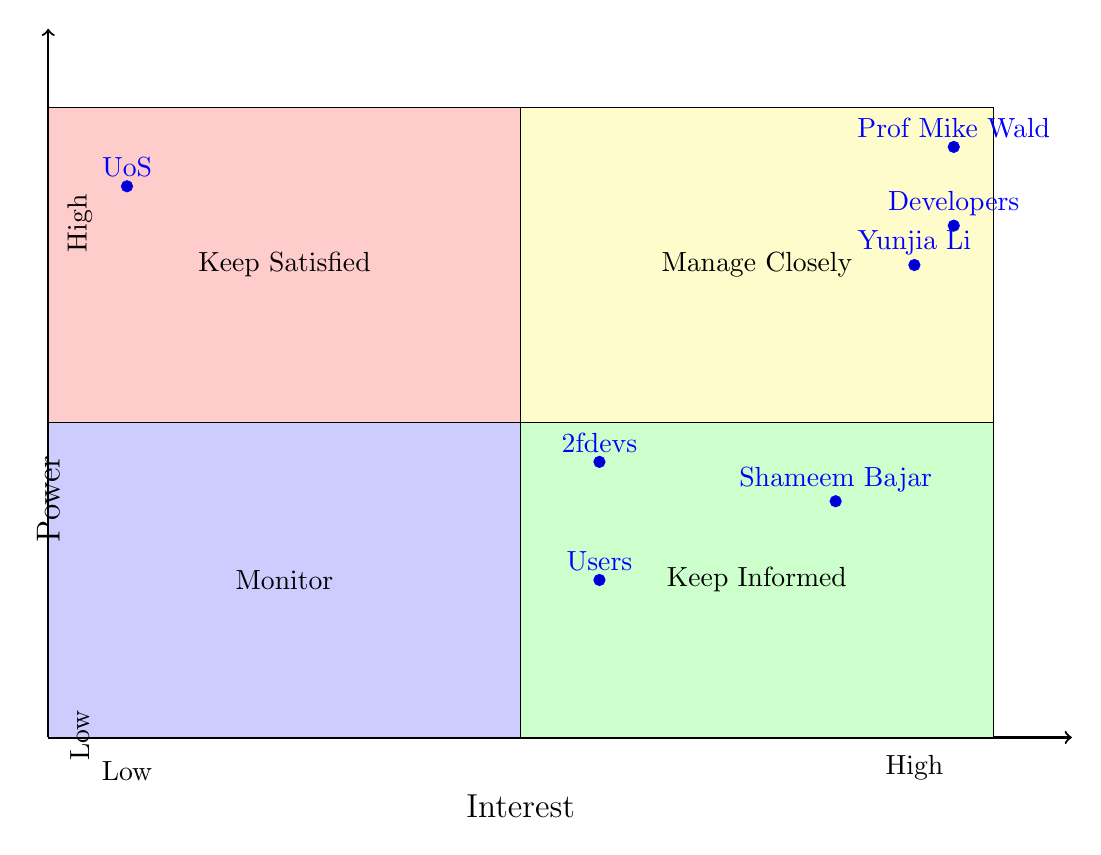
\begin{tikzpicture}[font=\rmfamily]
\draw [thick,->]  (0,0) -- coordinate (x axis mid) (13,0);
\draw [thick,->]  (0,0) -- coordinate (y axis mid) (0,9);
\filldraw[fill=blue!20!white, draw=black] (0,0) rectangle (6,4) node[pos=.5] {Monitor};
\filldraw[fill=green!20!white, draw=black] (6,0) rectangle (12,4) node[pos=.5] {Keep Informed};
\filldraw[fill=red!20!white, draw=black] (0,4) rectangle (6,8) node[pos=.5] {Keep Satisfied};
\filldraw[fill=yellow!20!white, draw=black] (6,4) rectangle (12,8) node[pos=.5] {Manage Closely};
%labels      
\node[xshift=-0.5cm, below=0.6cm] (xlabel) at (x axis mid) {{\large Interest}};
\node[rotate=90, left=0.8cm] (ylabel) at (y axis mid) {{\large Power}};
\begin{axis}[nodes near coords, xmin=0, xmax=13, ymin=0, ymax=9, width=13cm, height=9cm, axis x line=none, axis y line=none, scale only axis, enlargelimits=false]
\addplot+[only marks, point meta=explicit symbolic] coordinates { 
(11.5,7.5) [Prof Mike Wald] 
(7,3.5) [2fdevs] 
(10,3) [Shameem Bajar] 
(11,6) [Yunjia Li] 
(11.5,6.5) [Developers] 
(7, 2) [Users]
(1,7) [UoS]
 };
\end{axis}
\node[xshift=-5cm, above=0.2cm] at (xlabel) {Low};
\node[xshift=5cm, above=0.2cm] at (xlabel) {High};
\node[xshift=0.4cm,yshift=-3cm, rotate=90] at (ylabel) {Low};
\node[xshift=0.4cm,yshift=3.5cm, rotate=90] at (ylabel) {High};
\end{tikzpicture}
\caption{Stakeholder matrix for the project\label{fig:Stakeholder matrix}}
\end{figure}

Our supervisor and client, Professor Mike Wald, had the most interest and power in the project. As the project proposer it would be his ideas that would form the basis of the project.

Yunjia Li is the lead developer for the new version of Synote. As the aim of the project was to provide code that could be used within this he had a lot of interest in the project. His requirements would need to be taken into account to ensure interoperability between the two systems, which gave him power in the project.

Due to the nature of the project the developers on the project would be major stakeholders. All work would need to be evenly distributed to allow all members of the group to attain the same marks.

The University of Southampton sets the mark scheme and guidelines for the project. These would need to be satisfied to make the project successful.

2fdevs are the development team who created the \gls{Videogular} player. The project would be creating plugins for this player so would rely on certain attributes of \gls{Videogular} such as accessibility. 

Shameem Bajar is a 3rd year student who has an Individual Project based around this project. Her interest levels would be high as her work depends on the output of this project. 

The users would be interested in the outcome of the project as the decisions made will affect how easy the system is to use and whether all of the desired functionality is available.

Requirements from all stakeholders will be considered but any conflicts will be dealt with by prioritising the needs of the most influential party (closer to the top right of \autoref{fig:Stakeholder matrix}).

\section{Requirements Analysis}
\label{Section:Requirements Analysis}
Looking at the needs of all the stakeholders a set of requirements for the project were agreed.
\subsection{Functional Requirements}
\begin{requirement}[label=\textbf{F\arabic*}]
\item \textbf{Question types}  \label{Req:Question types} \hfill \\
The overlaid video player must be able to display single choice, multiple choice, range selector, rating and text based answer types.

\textit{The users to ask questions that require set responses.}
\item \textbf{Jumping to content} \label{Req:Jumping to content} \hfill \\ 
There should be a feature to jump to specific content if a question is answered incorrectly.

\textit{This is a method of giving instant feedback which was one of the things found to be important in the Previous Work (see \autoref{Chapter:Previous Work}).}
\item \textbf{Analytics events} \label{Req:Analytics events} \hfill \\ 
Video and question events should be emitted from the overlaid video player in order than analytics data can be calculated.

\textit{Analysis of existing work showed a lack of analysis of video usage behaviour so this would help facilitate new analysis.}
\item \textbf{Cuepoints} \label{Req:Cuepoints} \hfill \\ The locations of the questions should be marked visually on the scrub bar of the video.

\textit{Users wish to see where the questions are in the video.}
\item \textbf{Poll responses} \label{Req:Poll responses} \hfill \\ The responses to polls must be able to be sent to and recorded on a server to allow viewing of the results.

\textit{One of our client's requirements.}
\item \textbf{Instant feedback} \label{Req:Instant feedback} \hfill \\ Once a question or set of questions have been answered there must be a way of receiving instant feedback on performance.

\textit{Found to be important in the analysis of existing work.}
\end{requirement}

\subsection{Non-Functional Requirements}
\begin{requirement}[label=\textbf{N\arabic*}]
\item \textbf{Video player used} \label{Req:Video player used} \hfill \\ Videogular should be used as the video player with components written in AngularJS and HTML5.

\textit{One of Yunjia's requirements.}
\item \textbf{Standalone} \label{Req:Standalone} \hfill \\ The plugins created should be standalone code but still be easy to integrate into the new version of Synote.

\textit{One of the client's requirements.}
\item \textbf{Browser compatibility} \label{Req:Browser compatibility} \hfill \\ The overlaid video player must work on Internet Explorer, Firefox and Chrome 

\textit{One of the client's requirements.}
\item \textbf{Operating System Compatibility} \label{Req:OS compatibility} \hfill \\ The overlaid video player must work on Windows, OSX and Android.

\textit{One of the client's requirements.}
\item \textbf{Extensibility} \label{Req:Extensibility} \hfill \\ The overlaid video player must be extensible so that further features can be added. 

\textit{Makes incremental development easier for the developers and any missing features that are wanted for integration into Synote could easily be added.}
\item \textbf{Keyboard Accessibility}\label{Req:Keyboard accessibility} \hfill \\ The overlaid video player and authoring tool must be completely accessible to a keyboard-only user.

\textit{Users may not be able to use a mouse so the applications need to be accessible to a keyboard only user.}
\item \textbf{Use of colour}\label{Req:Use of colour} \hfill \\ Any colours used should be customisable.

\textit{Users may have visual impairments such as colour blindness so they may be able to use the application only if it is in certain colours.}
\item \textbf{User interface} \label{Req:User interface} \hfill \\ A Graphical User Interface (GUI) must be provided for the Authoring Tool so that non-technical users can create quizzes.

\textit{One of the client's requirements is to reduce the barrier to entry.}
\item \textbf{User friendliness} \label{Req:User friendliness} \hfill \\ To allow maximum use of these tools the use of all tools should not require extensive training.

\textit{One of the client's requirements is to reduce the barrier to entry.}
\item \textbf{Documentation} \label{Req:Documentation} \hfill \\ The plugins built should have usage examples documented to allow less technical users to implement their own system.

\textit{One of the client's requirements is to reduce the barrier to entry.}
\item \textbf{Testing Examples} \label{Req:Testing Examples} \hfill \\ The plugins built should have usage examples created as a proof of concept.

\textit{One of the client's requirements is ensure the framework is easy to integrate.}
\item \textbf{Server architecture} \label{Req:Server architecture} \hfill \\ Any server behaviour should be accessed by \gls{REST} calls with no requirement that all servers should be on the same host.

\textit{One of Yunjia's requirements to allow easier integration into Synote.}
\item \textbf{Scalability} \label{Req:Scalability} \hfill \\ All tools should scale when they are used by large numbers of people.

\textit{One of the client's requirements is to ensure performance does not degrade when use of the tools are scaled.}
\end{requirement}

\section{Modular Webserver Approach}
\label{Section:Modular Approach}

It is important for our project to be easily integrated into other projects, specifically we are looking to have it integrated into the latest version of Synote (see \autoref{Section:Synote}). To accomplish this we have designed the back end systems to ensure they can be run without depending on any other modules. All of the functionality will be able to be accessed by \gls{REST} calls as set out by \cref{Req:Server architecture}.

By abstracting all calls to using \gls{REST} this means that other services will be able to interact with out back end services in a language independent way which will also allow the application to be standalone (\cref{Req:Standalone}). To facilitate this we have had to ensure that all \gls{REST} responses are returned with a Cross-Origin header. This allows servers who are not on the same machine to be able to communicate with the \gls{REST} service.

These features will allow an external application to be able to run the webserver separately and communicate with our server side code. This ensures that the only dependency added by those that use our code will be that they need to be able to make \gls{REST} calls.

\section{System Architecture}

We decided on the following set of components, the interactions of which are shown in \autoref{fig:System architecture diagram}:

\begin{itemize}
	\item
		\textbf{Videogular Questions} will display questions over a \gls{Videogular} video player according to a quiz defined in a \gls{DF}. If the quiz contains polls, it will also send responses to a results server, and display results it receives back.
	\item
		\textbf{Videogular Analytics} will log events from \gls{Videogular} (e.g. when the user plays or pauses the video) and Videogular Questions (e.g. when the user answers a question) and send them to an analytics server.
	\item
		\textbf{Videogular Cuepoints} will display marks on the scrub bar indicating when questions will appear.
	\item
		The \textbf{results server} will receive responses from Videogular Questions and return the aggregated results on request.
	\item
		The \textbf{analytics server} will receive event logs from Videogular Analytics, and provide a separate Web front-end, the \textbf{analytics front-end}, which will display analysis of the events.
	\item
		\textbf{Videogular Heatmap} will overlay a heatmap onto the scrub bar of the \gls{Videogular} player, for visualisation of analytics results.
	\item
		An \textbf{authoring tool} will allow a user to create \glspl{DF} without having to write them manually.
\end{itemize}

\begin{figure}[h!]
\centering
\begin{tikzpicture}[
  font=\sffamily,
  every matrix/.style={ampersand replacement=\&,column sep=2cm,row sep=2cm},
  source/.style={draw,thick,rounded corners,fill=yellow!20,inner sep=.3cm},
  vg-plugin/.style={draw,thick,rounded corners,fill=yellow!20,inner sep=.3cm},
  videogular/.style={draw,thick,circle,fill=blue!20},
  process/.style={draw,thick,circle,fill=blue!20},
  sink/.style={source,fill=green!20},
  datastore/.style={draw,very thick,shape=datastore,inner sep=.3cm},
  server/.style={source,fill=green!20},
  dots/.style={gray,scale=2},
  to/.style={->,>=stealth',shorten >=1pt,semithick,font=\sffamily\footnotesize},
  between/.style={<->,>=stealth',shorten >=1pt,semithick,font=\sffamily\footnotesize},
  every node/.style={align=center}]

  % Position the nodes using a matrix layout
  \matrix{
    \node[vg-plugin] (cuepoints) {cuepoints};
      \&
      \& \node[vg-plugin] (questions) {questions};
      \& \node[server] (poll-server) {poll server}; \\

    \& \node[videogular] (videogular) {videogular}; \\

    \node[vg-plugin] (heatmap) {heatmap};
      \&
      \& \node[vg-plugin] (analytics) {analytics};
      \& \node[server] (analytics-server) {analytics server}; \\
  };

  \draw[between] (questions) --
      node[midway,above] {user responses}
      node[midway,below] {results} (poll-server);
  \draw[to] (questions) --
      node[midway,right] {user interactions}
      (analytics);
  \draw[to] (questions) --
      node[midway,above] {question times}
      (cuepoints);
  \draw[between] (analytics) --
      node[midway,above] {data}
      node[midway,below] {acks} (analytics-server);
  \draw[to] (analytics-server) to[bend left=15] node[midway,above] {events}
      node[midway,below] {level 1} (heatmap);
  \draw[between] (videogular) -- (cuepoints);
  \draw[between] (videogular) -- (analytics);
  \draw[between] (videogular) -- (questions);
  \draw[between] (videogular) -- (heatmap);
\end{tikzpicture}

\caption{System architecture diagram for the project \label{fig:System architecture diagram}}
\end{figure}

The results and analytics servers (including the analytics front-end) are examples only, and not themselves deliverables (see \autoref{Section:Deliverables}).

As the expected behaviour of our plugins will depend on the application they were used in, an example site would be required to test the other components.

\todo{Fix heatmap-analytics server arrow}
\todo{Change the box shape as well as colour for accessibility}

We decided to separate the server components as they do completely separate jobs, and because some deployments may use one but not the other. Similarly, Videogular Analytics is separate from Videogular Questions as it only depends on \gls{Videogular}. Videogular Cuepoints and Videogular Heatmaps are separate components as they can be used in other, completely unrelated, projects.

\section{Deliverables}
\label{Section:Deliverables}

The following set of deliverables was agreed in order to meet the requirements:

\begin{itemize}
\item Videogular Questions: a plugin for adding polls and questions to videos
\begin{itemize}
\item Source code, under the MIT licence
\item An example proof-of-concept website
\end{itemize}
\item Videogular Cuepoints: a plugin which displays informational marks on the scrub bar of a video
\begin{itemize}
\item Source code, under the MIT licence
\item Demonstration of usage in Videogular Questions example site
\end{itemize}
\item Videogular Analytics: a plugin for reporting of events within the Videogular player
\begin{itemize}
\item Source code, under the MIT licence
\item An API specification for Videogular Analytics
\item An example site showing basic usage of the analytics data collected from the plugin
\end{itemize}
\item Videogular Heatmap: a plugin which displays heat map information on the scrub bar of a video
\begin{itemize}
\item Source code, under the MIT licence
\item Demonstration of usage in Videogular Analytics example site
\end{itemize}
\item Authoring tool: a Web application to produce the \gls{DF} to be used with Videogular Questions
\begin{itemize}
\item Source code, under the MIT licence
\end{itemize}
\end{itemize}


\section{Testing}
\label{Section:Overall_Testing}

Software testing is necessary on projects of all sizes, especially on large projects such as this. To ensure quality throughout the project each part of the framework has been thoroughly tested.

One method of doing that is with example sites, this satisfies \cref{Req:Documentation} and \cref{Req:Testing Examples}. Due to the free-form nature of AngularJS's project structure we decided to sue one of the industry standards, angular-seed\footnote{\url{https://github.com/angular/angular-seed}}. angular-seed is a skeleton in which one can create AngularJS web apps. It includes two testing frameworks all ready set up, Karma and Jasmine. More details about Karma, Jasmine and other tests performed can be found in \autoref{Chapter: Testing}.

